\documentclass[11pt,a4paper]{report}

%%% Работа с русским языком
\usepackage{cmap}					% поиск в PDF
\usepackage{mathtext} 				% русские буквы в фомулах
\usepackage[T2A]{fontenc}			% кодировка
\usepackage[utf8]{inputenc}			% кодировка исходного текста
\usepackage[english,russian]{babel}	% локализация и переносы

\usepackage{fancyhdr}

\usepackage{lipsum}
\usepackage{etoolbox}
\usepackage{color}

% Code in Latex
\usepackage{listings}



%%% Работа с картинками
\usepackage{graphicx}  % Для вставки рисунков
\graphicspath{{images/}}  % папки с картинками
\setlength\fboxsep{3pt} % Отступ рамки \fbox{} от рисунка
\setlength\fboxrule{1pt} % Толщина линий рамки \fbox{}
\usepackage{wrapfig} % Обтекание рисунков и таблиц текстом
\usepackage[export]{adjustbox}
\usepackage{subcaption}
\usepackage{float}

%%% Дополнительная работа с математикой
\usepackage{amsmath,amsfonts,amssymb,amsthm,mathtools} % AMS
\usepackage{icomma} % "Умная" запятая: $0,2$ --- число, $0, 2$ --- перечисление
\usepackage{systeme}

\usepackage{tabularx}
\usepackage{tikz-cd}



\patchcmd{\maketitle}
  {\end{titlepage}}
  {\thispagestyle{titlepagestyle}\end{titlepage}}
  {}{}

\fancypagestyle{titlepagestyle}
{
   \fancyhf{}
   \fancyfoot[C]{3 курс, 3 группа}
   \renewcommand{\headrulewidth}{0 mm}
}

\pagestyle{plain}

\title{Введение в нечеткое моделирование \protect \\ Вариант 2}
\author{Снопов П.М.}
\date{2020}
\thispagestyle{titlepagestyle}


\renewcommand{\thesection}{\arabic{section}}
\newcommand{\insref}[1]{рис. \ref{#1}}

\begin{document}
	\maketitle
	\tableofcontents
	\newpage
	\section{Постановка задачи}
	Пусть задана функция от двух переменных:
	\[
		F(x_1,x_2) = 10 \cdot \frac{x_1 + x_1x_2}{x_1 - 2x_1x_2 + x_2},
	\]
	где $ x_1, x_2 \in [0,1] $, $ F(x_1,x_2) \in [0,10] $.
	\newline
	Для приближенного описания функции введена лингвистическая шкала:
	\begin{center}
		$N$ -- {\it незначительный}, \\
		$VS$ -- {\it очень малый}, \\
		$S$ -- {\it малый}, \\
		$M$ -- {\it средний}, \\
		$L$ -- {\it большой}, \\
		$VL$ -- {\it очень большой}, \\
		$P$ -- {\it значительный}.
	\end{center}
	База правил, описывающая зависимость выходной переменной от входных, представлена в следующей таблице:
	\begin{table}[!hbtp]
		\centering
		\begin{tabular}{|c|c|c|c|c|c|c|c|}
			\hline
			& N & VS & S  & M  & L  & VL & P \\ \hline
			N  & N & N  & N  & N  & N  & N  & N \\ \hline
			VS & P & M  & S  & VS & VS & N  & N \\ \hline
			S  & P & L  & M  & S  & VS & VS & N \\ \hline
			M  & P & VL & L  & M  & S  & VS & N \\ \hline
			L  & P & VL & VL & L  & M  & S  & N \\ \hline
			VL & P & P  & VL & VL & L  & M  & N \\ \hline
			P  & P & P  & P  & P  & P  & P  & P \\ \hline
		\end{tabular}
	\end{table}
	\newline
	В пакете $Matlab$ построить поверхность "вход-выход". Как изменяется поверхность в зависимости от типа функции принадлежности переменных?
	\newpage
	\section{Решение}
	\subsection{Треугольная функция приндлежности}
	Так как для описания функции введена лингвистическая шкала, то будем пользоваться алгоритмом Мамдани. Выберем в качестве функции принадлежности термов треугольную функцию принадлежности(\insref{fig:trimf}).
	\begin{figure*}[!hbtp]
		\centering
		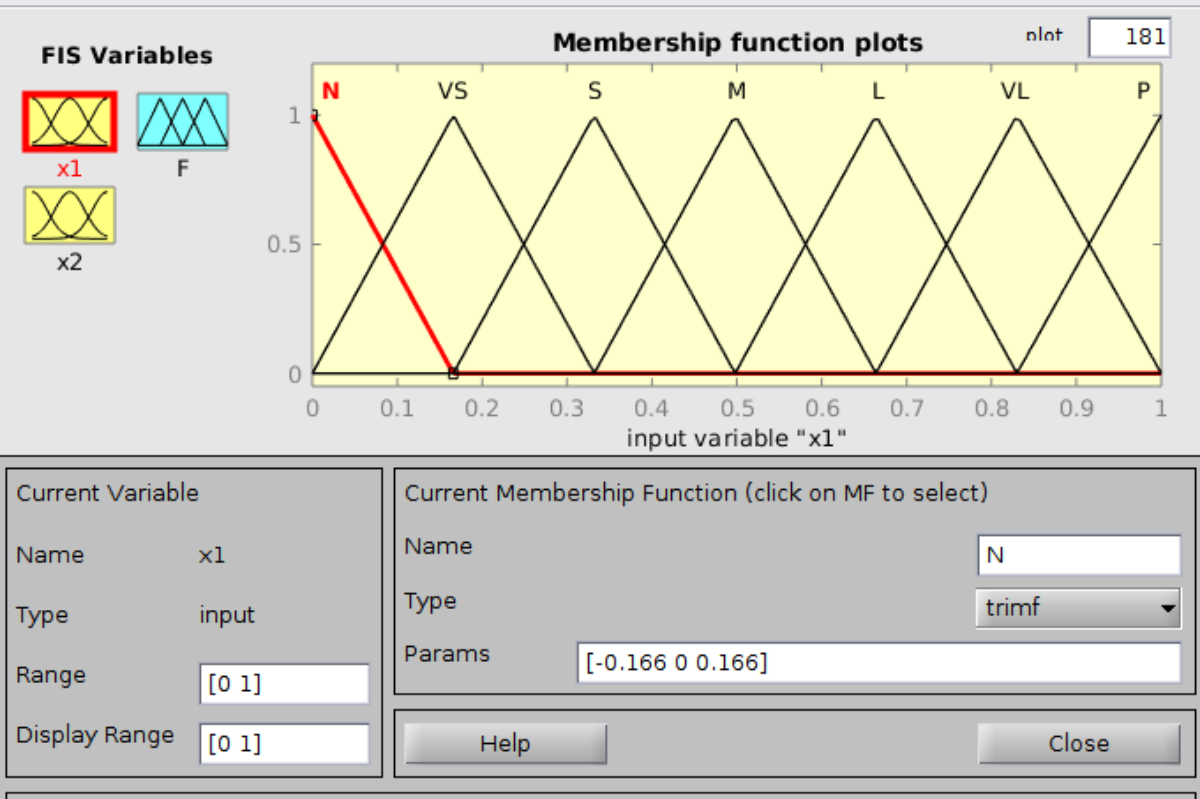
\includegraphics[width=\linewidth]{trimf.png}
		\caption{Переменная $x_1$, заданная треугольной функцией принадлежности}
		\label{fig:trimf}
	\end{figure*}
	\newline
	Зададим базу правил(\insref{fig:rules}) и получим необходимую поверхность(\insref{fig:trim_surf}).
	\begin{figure*}[!hbtp]
		\centering
		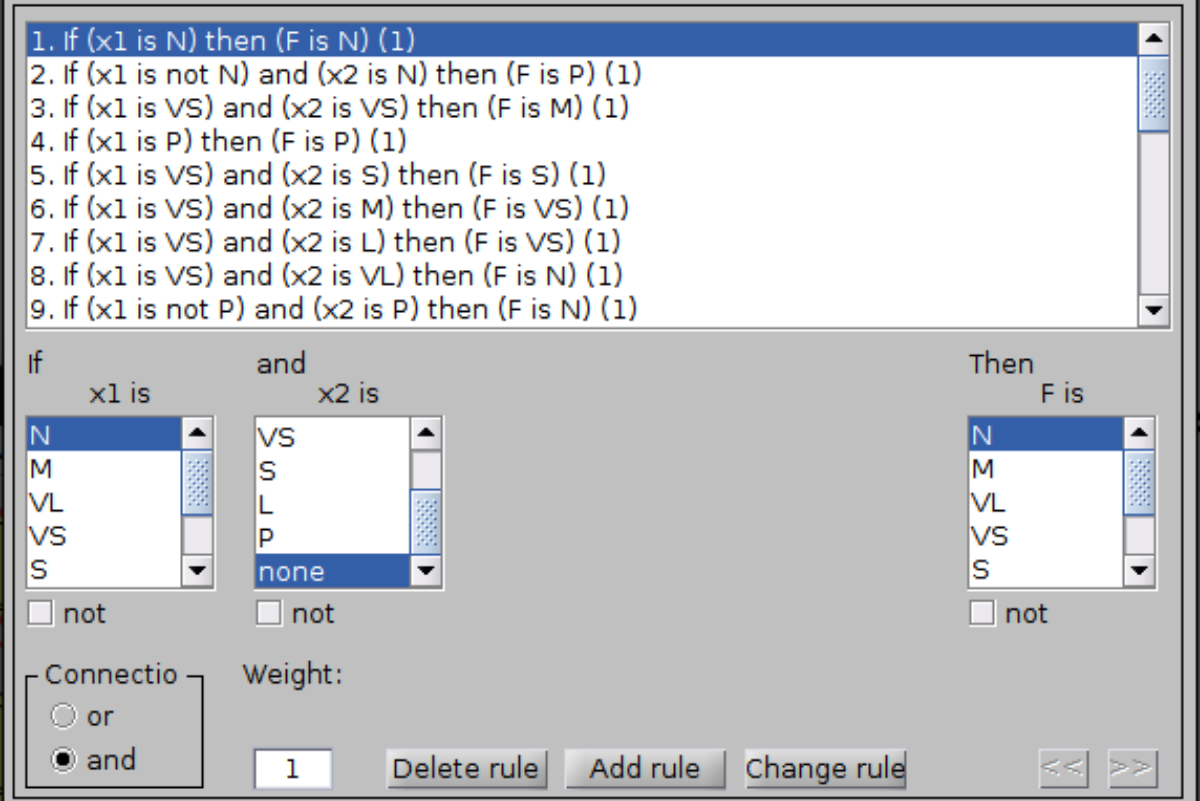
\includegraphics[width=\linewidth]{rules.png}
		\caption{База правил}
		\label{fig:rules}
	\end{figure*}
	\begin{figure*}[!hbtp]
		\centering
		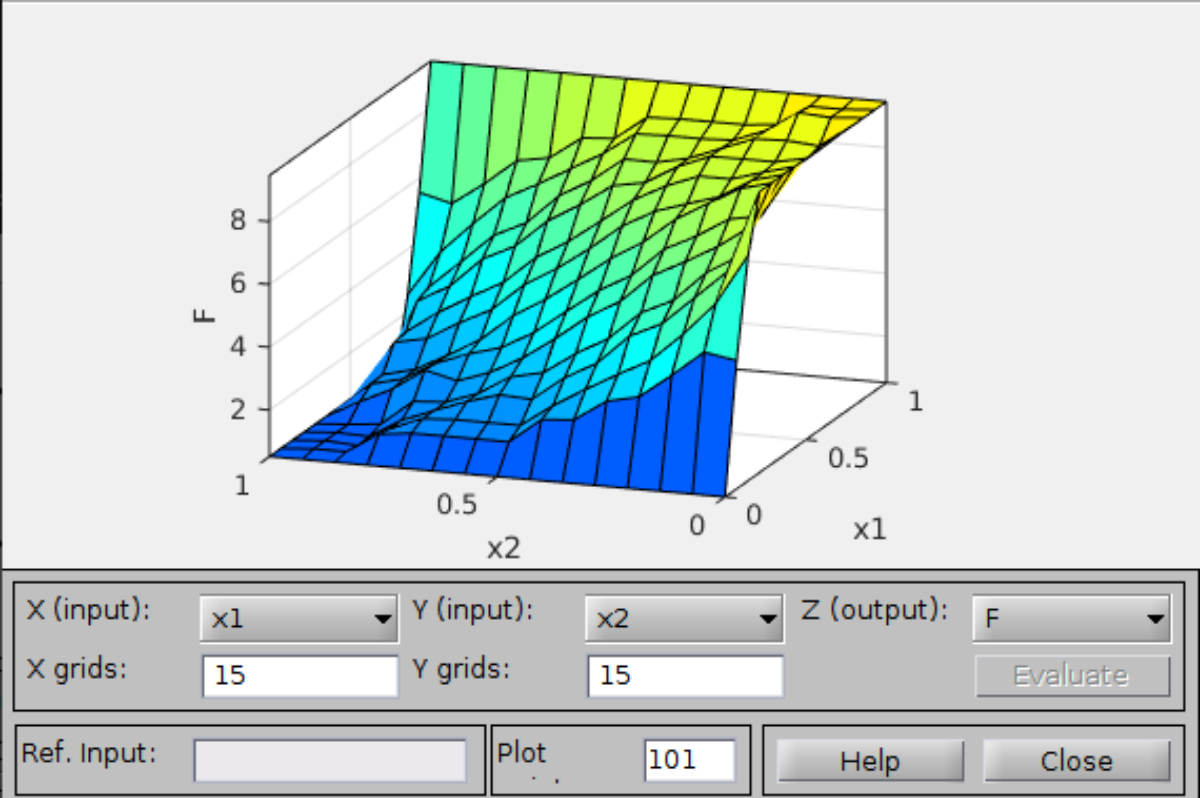
\includegraphics[width=\linewidth]{trim_surf.png}
		\caption{Поверхность, полученная с использованием треугольной функцией принадлежности}
		\label{fig:trim_surf}
	\end{figure*}
	\newline
	В свою очередь окно визуализации нечеткого логического вывода выглядит так(\insref{fig:logoutput_trimf}).
	\begin{figure*}[!hbtp]
		\centering
		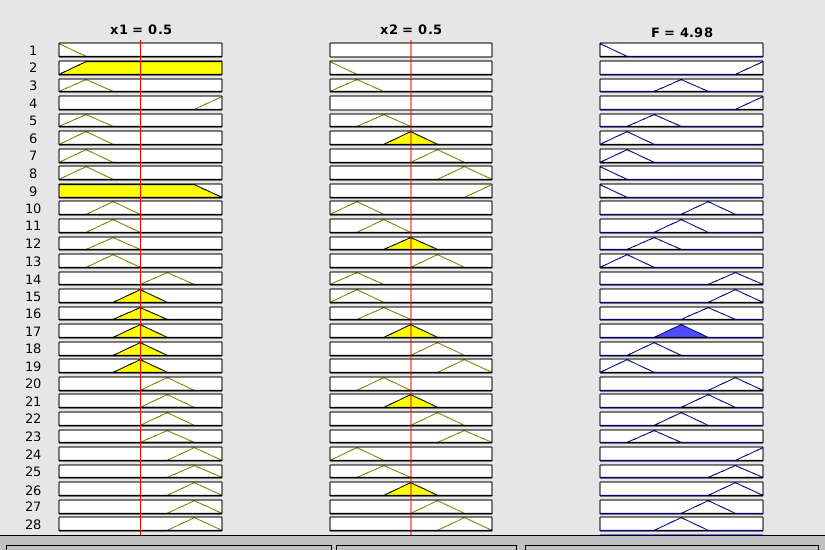
\includegraphics[width=\linewidth]{logoutput_trimf.png}
		\caption{Окно визуализации нечеткого логического вывода}
		\label{fig:logoutput_trimf}
	\end{figure*}
	\newpage
	\subsection{Гауссова функция приндлежности}
	Теперь выберем в качестве функции принадлежности термов гауссову функцию принадлежности(\insref{fig:gaussmf}).
	\begin{figure*}[!hbtp]
		\centering
		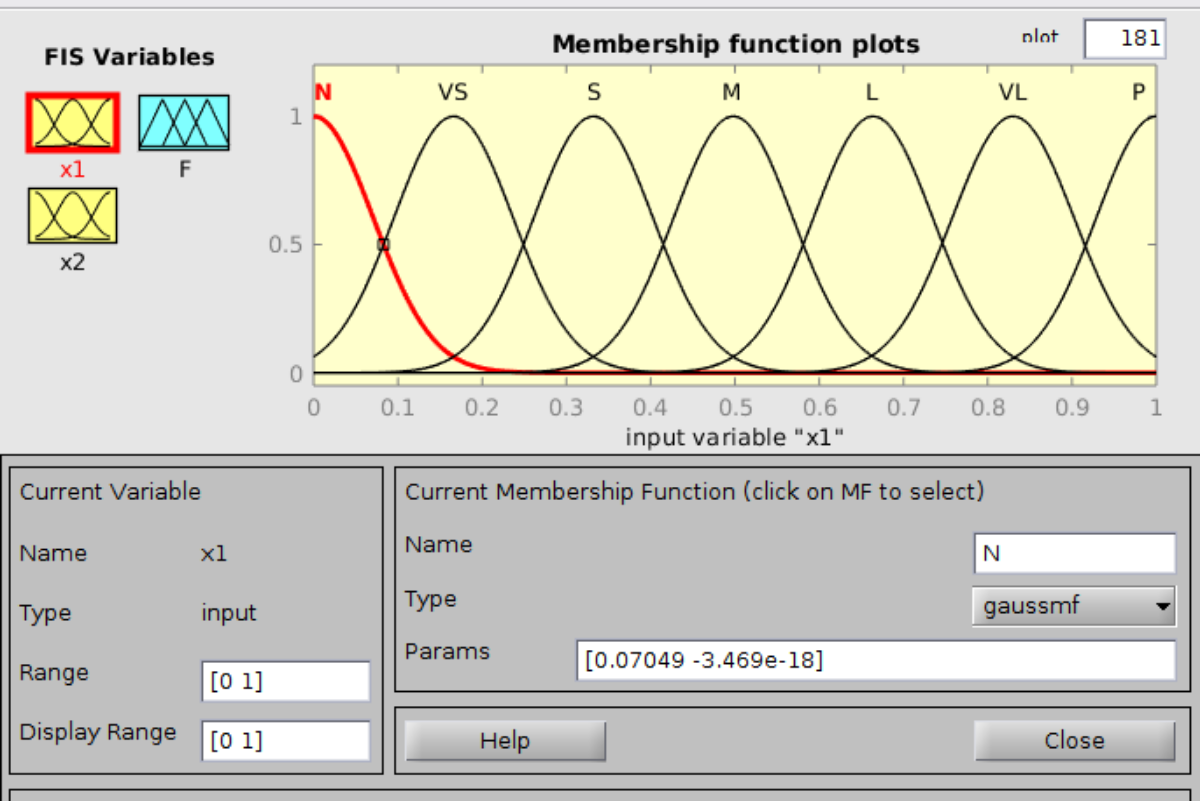
\includegraphics[width=\linewidth]{gaussmf.png}
		\caption{Переменная $x_1$, заданная гауссовой функцией принадлежности}
		\label{fig:gaussmf}
	\end{figure*}
	В таком случае поверхность будет иметь вид(\insref{fig:gauss_surf}). Как можно заметить, различия между двумя представленными поверхностями минимальны.
	\begin{figure*}[!hbtp]
		\centering
		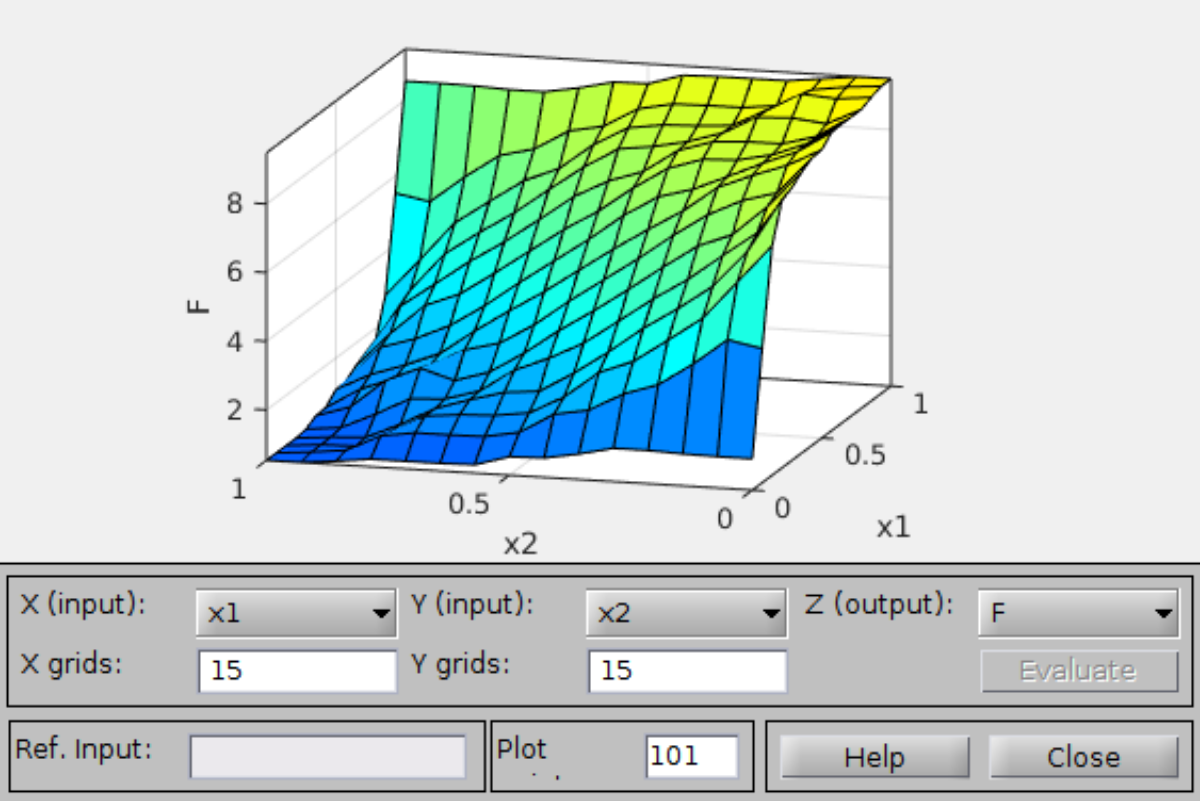
\includegraphics[width=\linewidth]{gauss_surf.png}
		\caption{Поверхность, полученная с использованием гауссовой функцией принадлежности}
		\label{fig:gauss_surf}
	\end{figure*}
	\newpage
	В свою очередь окно визуализации нечеткого логического вывода выглядит так(\insref{fig:logoutput_gaussmf}).
	\begin{figure*}[!hbtp]
		\centering
		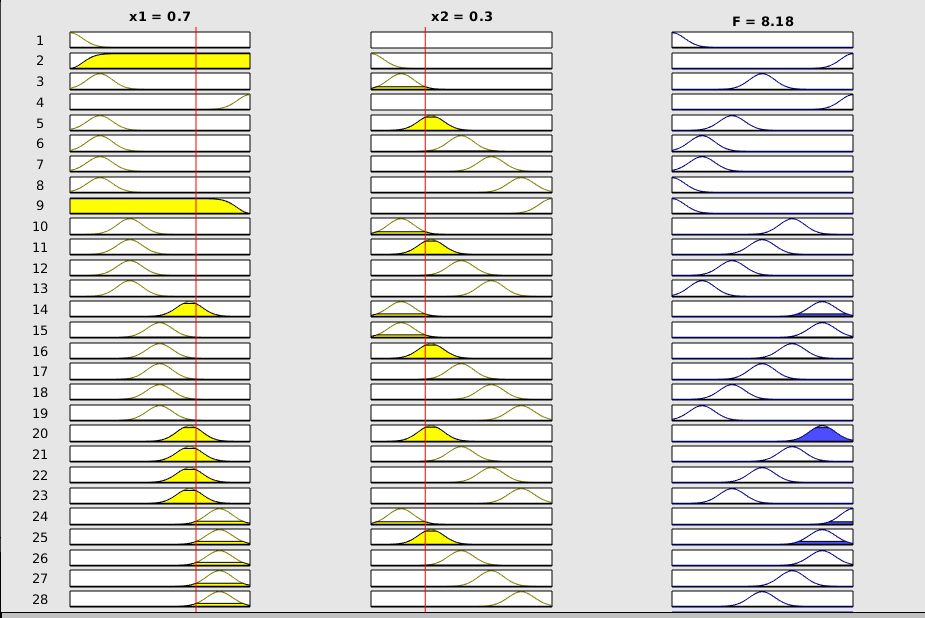
\includegraphics[width=\linewidth]{logoutput_gaussmf.png}
		\caption{Окно визуализации нечеткого логического вывода}
		\label{fig:logoutput_gaussmf}
	\end{figure*}
\end{document}
